\documentclass{article}
\usepackage{graphicx}
\usepackage[]{mdframed}
\usepackage{tabularx}
\usepackage{subfig}
\usepackage{placeins}
\usepackage{float}

\graphicspath{ {./images/} }
\usepackage[a4paper, total={6in, 8in}]{geometry}


\author{Sidharth Babu, SNB2593 \and Tianda Huang, TH32684}
\title{ECE 361E: Homework 1}

\begin{document}
\begin{mdframed}
    \maketitle
\end{mdframed}

\section{Problem 1}
\subsection{Question 2}
Loss Plot:
\newline
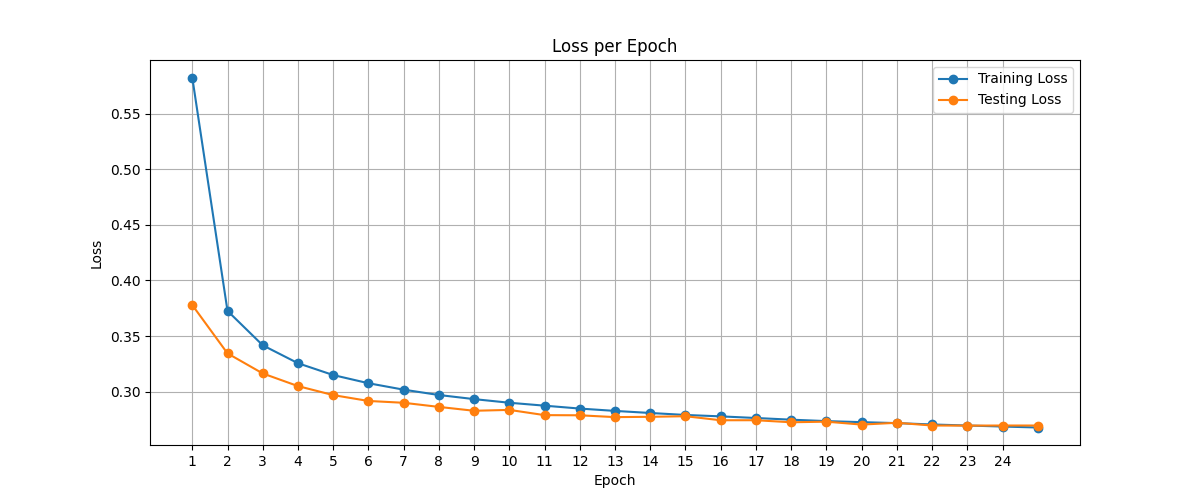
\includegraphics[width=\textwidth]{p1_lossplot.png}
\newline
Accuracy Plot:
\newline
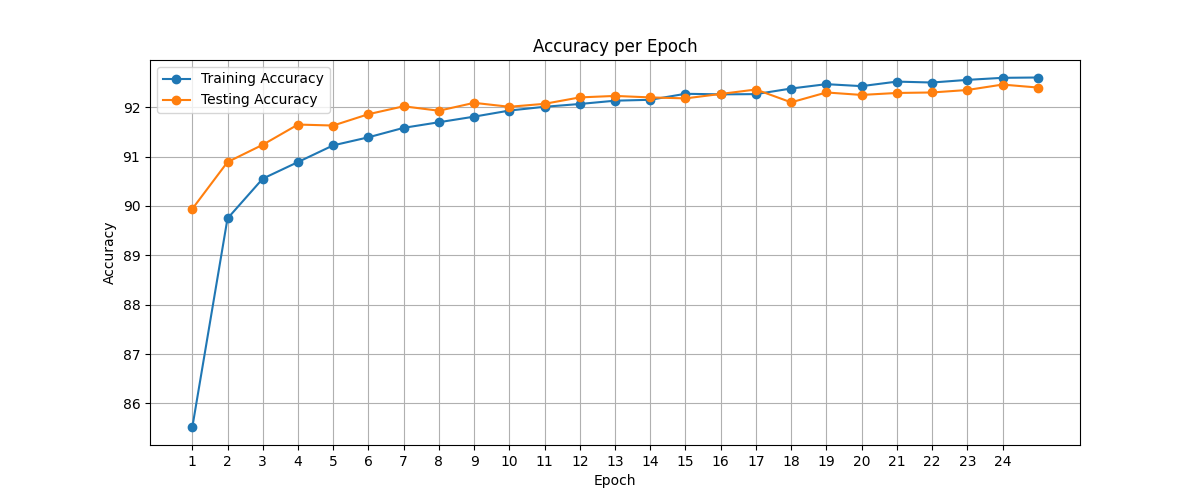
\includegraphics[width=\textwidth]{p1_accplot.png}
\subsection{Question 3}
\begin{center}
    \begin{tabularx}{\textwidth} { 
        | >{\centering\arraybackslash}X 
        | >{\centering\arraybackslash}X 
        | >{\centering\arraybackslash}X 
        | >{\centering\arraybackslash}X 
        | >{\centering\arraybackslash}X 
        | >{\centering\arraybackslash}X | }
       \hline
       Training Accuracy & Testing Accuracy & Total Training Time (s) & Total Inference Time (s) & Average Inference Time (ms) & GPU memory during training (MB) \\
      \hline
      92.60 & 92.40 & 188.11 & 0.52 & 0.0522 & 655\\
      \hline
    \end{tabularx}
\end{center}

\section{Problem 2}
\subsection{Question 1}
Loss Plot:
\newline
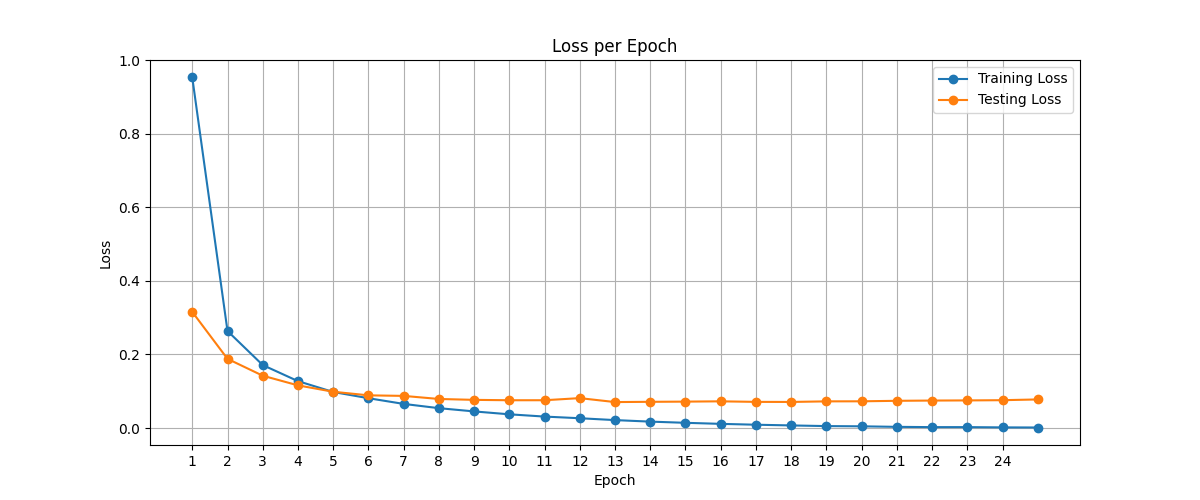
\includegraphics[width=0.9\textwidth]{p2_1_lossplot.png}
\newline
Accuracy Plot:
\newline
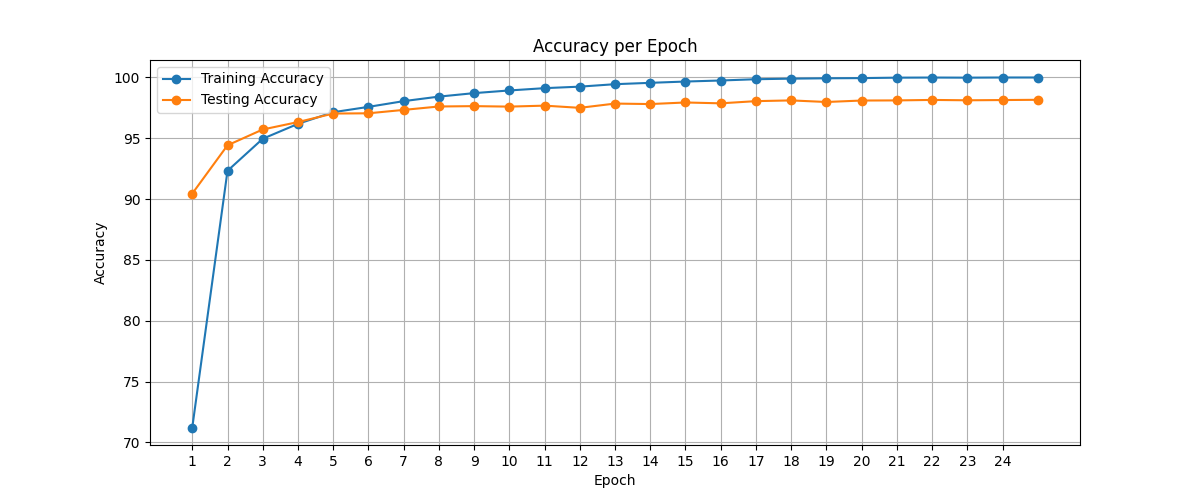
\includegraphics[width=0.9\textwidth]{p2_1_accplot.png}
\newline
This model does overfit slightly. Past epoch 5, we can see that the training accuracy exceeds the test accuracy, and the training loss is less than the test loss. We also see that the discrepancy between the two grows over time. This is a sign of overfitting. However, the model does not overfit much, as the test loss and accuracy are not sacrificed significantly for the training accuracy and loss. It just means that the model continues to get better on the training set, but does not gain any additional ability to generalize to the test set, as the test loss and accuracies stabilize.

\subsection{Question 2}
    \begin{figure}[H]
        \noindent
        \makebox[\textwidth]{
            \subfloat{
                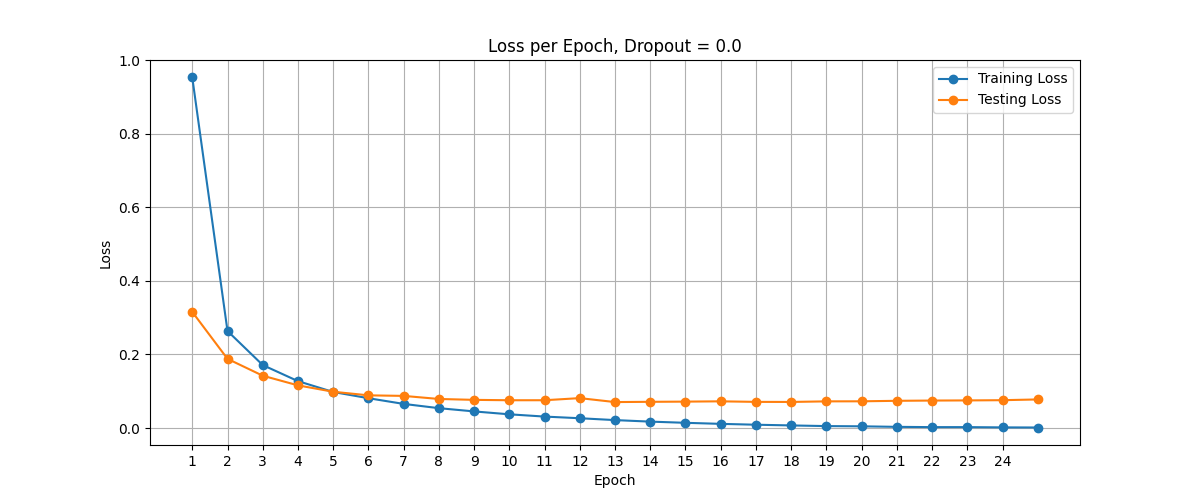
\includegraphics[width=0.7\textwidth]{lossplot_0d0.png}
            }
            \newline
            \subfloat{
                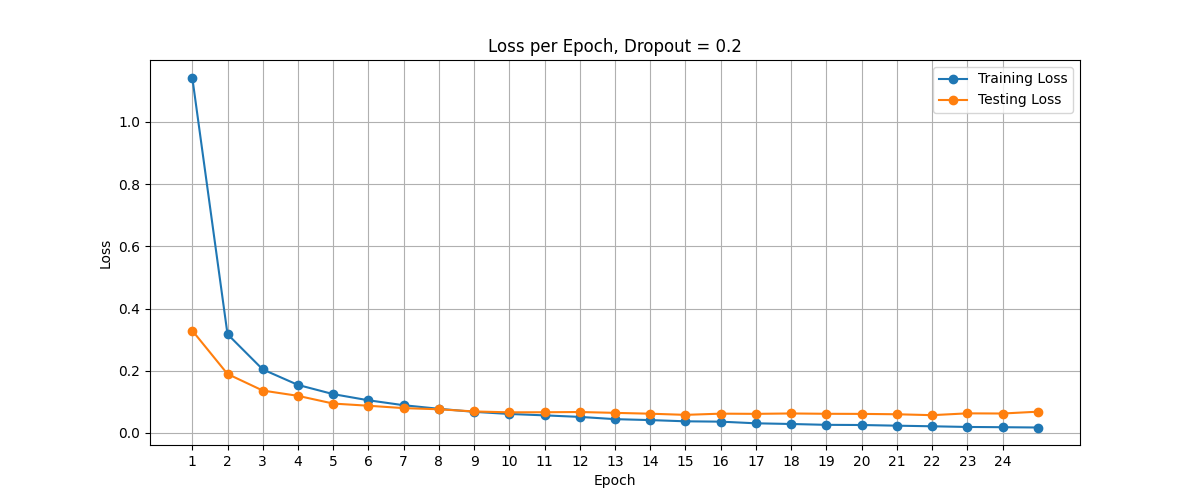
\includegraphics[width=0.7\textwidth]{lossplot_0d2.png}
            }
        }
        \label{fig1}
    \end{figure}

    \begin{figure}[H]
        \noindent
        \makebox[\textwidth]{
            \subfloat{
                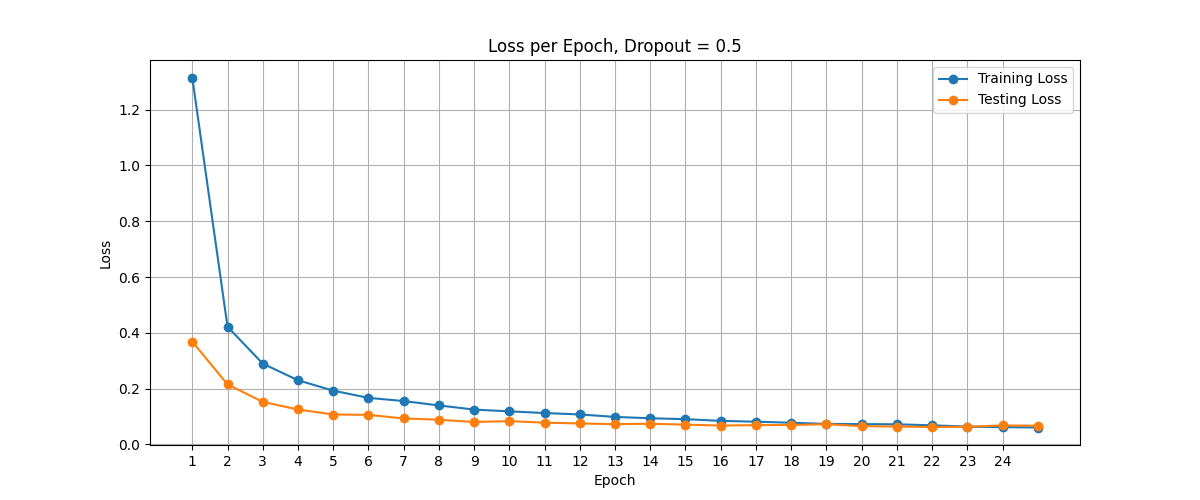
\includegraphics[width=0.7\textwidth]{lossplot_0d5.png}
            }
            \newline
            \subfloat{
                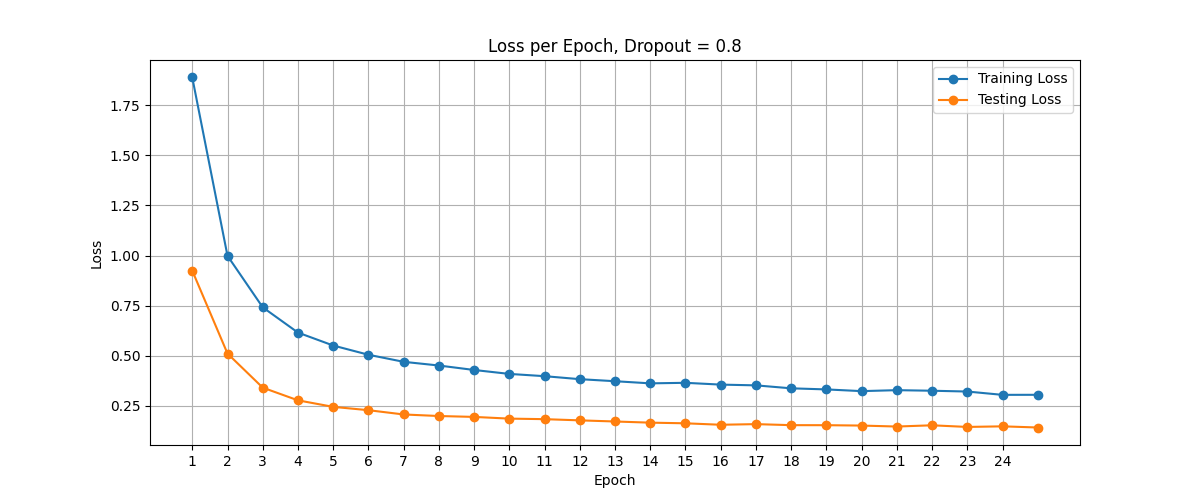
\includegraphics[width=0.7\textwidth]{lossplot_0d8.png}
            }
        }
        \label{fig2}
        \caption{Loss Plots for Different Dropout Fractions}
    \end{figure}

    \begin{center}
        \begin{tabularx}{\textwidth}{
            | >{\centering\arraybackslash}X 
            | >{\centering\arraybackslash}X 
            | >{\centering\arraybackslash}X |}
            \hline
            Dropout Fraction & Training Loss & Testing Loss\\
            \hline
            0.0 &  0.0015 & 0.0777 \\
            \hline
            0.2 &  0.0176 & 0.0684\\
            \hline
            0.5 &  0.0607 & 0.0671 \\
            \hline
            0.8 &  0.3045 & 0.1412 \\
            \hline
        \end{tabularx}
    \end{center}
The best dropout fraction is 0.5. The no dropout model has a significantly divergent training and test loss, with the test loss being much worse. This indicates an overfit model. \\
The 0.2 dropout model has a similar divergence, but on a much smaller scale. It has almost the same testing loss, but is slightly worse, indicating that it is close but not as good at generalizing as the 0.5 dropout model. The 0.8 dropout model has the opposite problem, with a significantly higher training and testing loss, indicating a severely underfit model. \\
These results, especially the 0.2 vs 0.5 case, shows that the dropout helps against overfitting in the model, though the 0.8 case shows that too much dropout causes loss to increase. The loss in accuracy can be explained by the large dropout resulting in too little complexity to fit the problem.


\subsection{Question 3}

\begin{center}
    \begin{tabularx}{\textwidth} { 
        | >{\centering\arraybackslash}X 
        | >{\centering\arraybackslash}X 
        | >{\centering\arraybackslash}X
        | >{\centering\arraybackslash}X 
        | >{\centering\arraybackslash}X | }
        \hline
        Dropout Fraction & Training Accuracy & Testing Accuracy & Total Training time (s)  & First Epoch when the model reaches 96 \% training accuracy\\
        \hline
        DF=0.5 & 98.20 & 98.19 & 4.26 & 8\\
        \hline
        DF=0.5 + norm & 98.54 & 98.38 & 4.31 & 6\\
        \hline
    \end{tabularx}
\end{center}

We can see that the normalized version of the model reaches 96\% training accuracy in 6 epochs, while the non-normalized version reaches 96\% training accuracy in 8 epochs. This is a significant improvement, and shows that normalization is a useful technique to speed up training. It also has a higher accuracy on both the training and testing set, showing that it is easier for the model to learn with the dataset properly with normalization. This is likely due to the fact that normalization smoothes out any statistical noise in the data, and enhances the model's ability to generalize. While the performance increase is not significant due to MNIST being quite uniform, it can be very useful for other datasets.

\section{Problem 3}
\subsection{Questions 1 and 2}
\begin{center}
    \begin{tabularx}{\textwidth} { 
        | >{\centering\arraybackslash}X 
        | >{\centering\arraybackslash}X 
        | >{\centering\arraybackslash}X 
        | >{\centering\arraybackslash}X 
        | >{\centering\arraybackslash}X 
        | >{\centering\arraybackslash}X | }
       \hline
       Model Name & MACs & FLOPs & \# Parameters & Model Size (MB) & Saved Model Size (KB) \\
      \hline
      SimpleCNN & 3869824 & 7739648 & 50,186 & 0.51 & 197\\
      \hline
      SimpleCNN + BatchNorm & 3894912 & 7789824 & 50,250 & 0.56 & 199\\
      \hline
    \end{tabularx}
\end{center}

The saved model size is many times smaller than the in-memory model size. This is due to a combination of data compression with the saved format and eliminating the added space of model metadata. Additionally, in-memory tensors and other model elements are located sparsely in memory to increase performance with the model's memory access patterns; this sparsity can be eliminated when saving the model to disk.

\begin{figure}[H]
    \noindent
    \makebox[\textwidth]{
        \subfloat{
            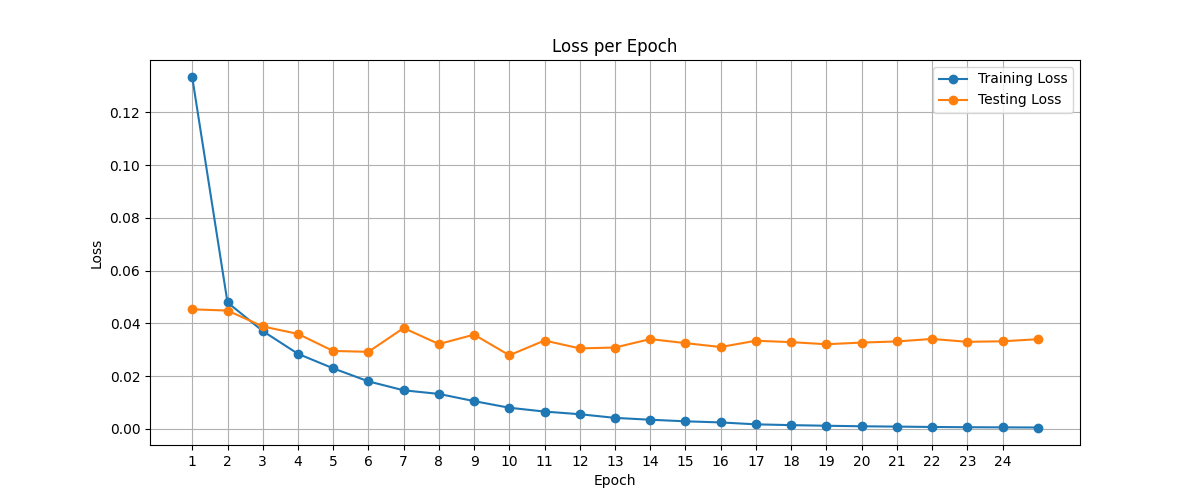
\includegraphics[width=0.7\textwidth]{p3_2_lossplot.png}
        }
        \newline
        \subfloat{
            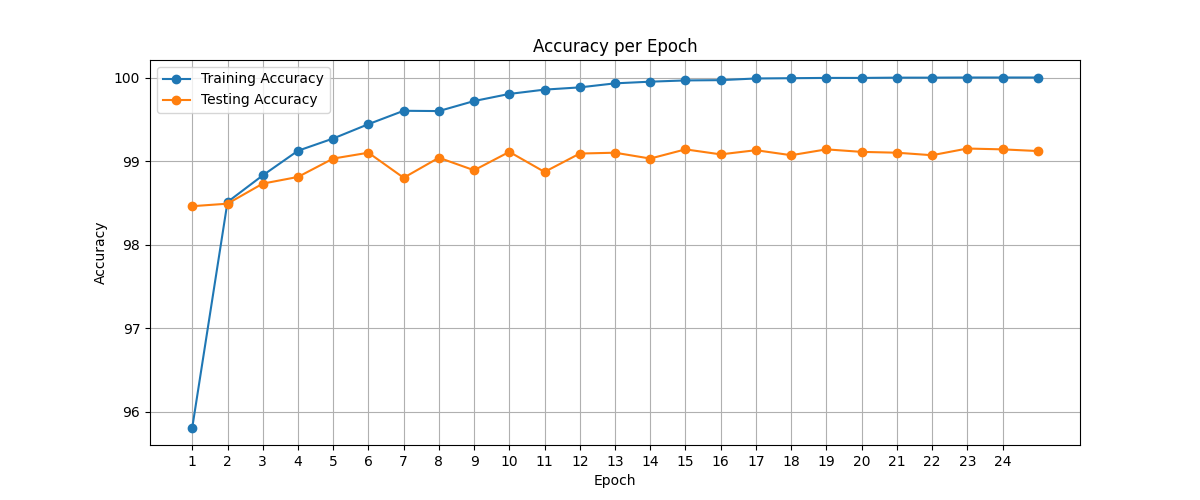
\includegraphics[width=0.7\textwidth]{p3_2_accplot.png}
        }
    }
    \label{fig3}
    \caption{Loss and Accuracy plots of custom CNN}
\end{figure}

\subsection{BONUS Question 3}
We retained most of SimpleCNN's architecture, but added a batch normalization layer before the second convolutional layer. This follows an intuition developed in the previous problem where we saw results improve with a normalized input. By adding a batch normalization layer in the middle of the network, we can mitigate covariate shift internal to the network, and cause the network to generalize better. This is reflected in the results, as it performs significantly better than the best of the previous models, with a training loss of almost 0.0005 and a test loss of 0.0340. While there is some (small) difference between the training loss and the test loss, indicating some overfitting to the train set, it retains extremely good general performance. This is likely due to the high uniformity of the MNIST dataset making it difficult to severely overfit. 


\end{document}
